%+----------------------------------------------------------------------------+
%| SLIDES: 
%| Chapter: Results of the paper with M. Spera
%| Author: Antonio miti
%| Event: PHD preliminary Defence
%+----------------------------------------------------------------------------+

%- HandOut Flag -----------------------------------------------------------------------------------------
\newif\ifHandout

%- D0cum3nt ----------------------------------------------------------------------------------------------
\documentclass[beamer,10pt]{standalone}   
%\documentclass[beamer,10pt,handout]{standalone}  \Handouttrue  

%- HandOut Flag -----------------------------------------------------------------------------------------
\ifHandout
	\setbeameroption{show notes} %print notes   
\fi
	
%- Packages ----------------------------------------------------------------------------------------------
\usepackage{custom-style}

%--Beamer Style-----------------------------------------------------------------------------------------------
\usetheme{toninus}



%---------------------------------------------------------------------------------------------------------------------------------------------------
%- D0cum3nt ----------------------------------------------------------------------------------------------------------------------------------
\begin{document}
%------------------------------------------------------------------------------------------------


\begin{frame}{Applications to hydrodynamics and knot theory}\label{frame:hydro1}
	\begin{columns}[T] % align columns
	\begin{column}{.4\textwidth}
		\vspace{.5em}
		\centering
			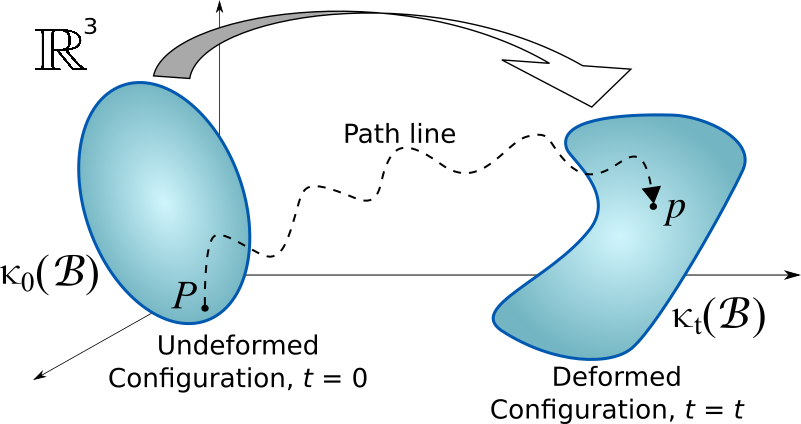
\includegraphics[width=\linewidth]{Pictures/Figure_continuum}
	\end{column}
	%
	\hfill
	%
	\begin{column}{.6\textwidth}
		\scalebox{.8}{%
			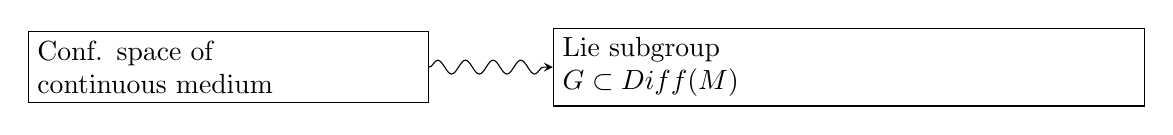
\begin{tikzpicture}[
				node distance=0.65\linewidth,
				]
				\node [text width=0.4\linewidth,rectangle,draw] (lhs) {Conf. space of\\ continuous medium};
				\node [text width=0.6\linewidth, rectangle,draw,right of=lhs] (rhs) {Lie subgroup \\$G \subset Diff(M)$};
				\draw[-stealth,decorate,decoration={snake}] (lhs) -- (rhs);
			\end{tikzpicture}
		}		
		Examples:
		\scalebox{.8}{%		
		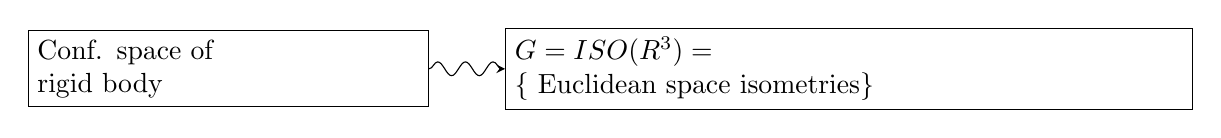
\begin{tikzpicture}[
			node distance=0.65\linewidth,
			]
			\node [text width=0.4\linewidth,rectangle,draw] (lhs) {Conf. space of\\ rigid body};
			\node [text width=0.7\linewidth,rectangle,draw,right of=lhs] (rhs) {$G=ISO(\mathbb{R}^3)=$\\ $\{$
				Euclidean space isometries$\}$};
			\draw[-stealth,decorate,decoration={snake}] (lhs) -- (rhs);
		\end{tikzpicture}
		}
		\scalebox{.8}{%
		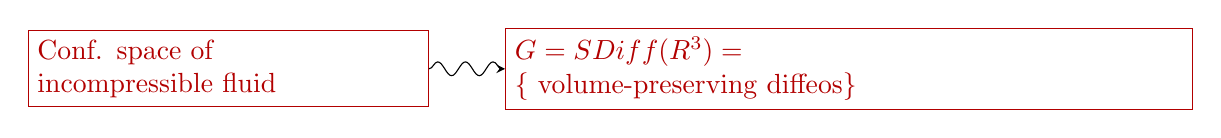
\begin{tikzpicture}[
			node distance=0.65\linewidth,
			]
			\node [text width=0.4\linewidth,red!70!black,rectangle,draw] (lhs) {Conf. space of\\ incompressible fluid};
			\node [text width=0.7\linewidth,red!70!black,rectangle,draw,right of=lhs] (rhs) {$G= SDiff(\mathbb{R}^3)=$\\ $\{$
				volume-preserving diffeos$\}$};
			\draw[-stealth,decorate,decoration={snake}] (lhs) -- (rhs);
		\end{tikzpicture}
		}
	\end{column}%
	\end{columns}
	\pause
	\vfill
	We consider the following setting:
	
	\begin{itemize}%[<+->]
		\item[$\bullet$]2-plectic manifold: 
		\vspace{-1em} 
			$$M=(\mathbb{R}^3,\nu = dx\wedge dy\wedge dz)$$
			\vspace{-.8em}\pause
		\item[$\bullet$]$\infty$-dim. Lie algebra (\emph{ideal fluid velocities}): \vspace{-1em}
			$$\mathfrak{g}:= sdiff_0(\mathbb{R}^3) = \left\lbrace  X \in \mathfrak{X}(\mathbb{R}^3) ~\left\vert~ 
		  		\substack{ div X = 0, \\ \textrm{\emph{ rapidly vanishing at }}\infty} \right\rbrace \right.$$
		  	\vspace{.2em}\pause
		\item[$\bullet$] Multisymplectic Lie algebra action:
			\vspace{-1em} 
			$$\mathfrak{g}= sdiff_0 \hookrightarrow  \mathfrak{X}(\mathbb{R}^3)$$
\end{itemize}		
	\pause
	\vfill
	\begin{center}
	\tcbox[enhanced,frame hidden,borderline={0.5pt}{0pt}{red,dashed}]{	
		\alert{
		\faQuestionCircle \qquad
			{Does $sdiff_0 \circlearrowleft (\mathbb{R}^3,\nu = dx\wedge dy\wedge dz)$ admit an HCMM?}	
		\qquad \faQuestionCircle		
		}
	}
	\end{center}

\end{frame}
\note[itemize]{
	\item We are working in the setting of \emph{geometric continuum mechanics} .\\
		Recall that the configuration space of a continuum object is encoded via diffeomorphisms. In the case of an incompressible fluid is encoded via volume-preserving diffeomorphisms.
	\item (Configution space is the set of spatial displacement of a mechanical systems. These are different from the \emph{physical states}.
	\item Such manifolds are infinite dimensional. Particular caution has to be taken in defining the smooth structure in this case.
	\item However, what really matters in the construction of a moment map is the infinitesimal action, i.e. the Lie algebra. In our case, the infinitesimal action to be considered is via divergence-free vector fields.
	\item (Notation): In the following M will be the 3 dimensional Euclidean Space.
	\item The simple but crucial observation is that the standard volume form on the euclidean space is a multisymplectic form.


}



%---------------------------------------------------------------------------------------------------------------------------------------------------
\begin{frame}{A Hydrodynamical HCMM}\label{frame:hydro2}
	\begin{columns}
		\begin{column}[c]{.5\linewidth}
		  	\begin{itemize}
		  		\item The observables are  $$L= \Omega^1_{\textrm{ham}}(\mathbb{R}^3)\oplus\Omega^0(\mathbb{R}^3)$$
		  		\item \hyperlink{frame:hydromomap-details}{HCMM consists of a pair of functions}:
					\begin{align*}
						f_1 &\colon \mathfrak{g} \rightarrow \Omega^1_{\textrm{ham}}(\mathbb{R}^3) \\
						f_2 &\colon \mathfrak{g}\wedge\mathfrak{g} \rightarrow C^\infty(\mathbb{R}^3)
					\end{align*}	
		  	\end{itemize}
		\end{column}	
	  	\hfill  	
		\begin{column}[c]{.5\linewidth}
  		\includestandalone[width=\textwidth]{Pictures/Figure_Euclid_Trigger}
 	 	\end{column}
 	 \end{columns}


	\pause
\tcbset{colback=white,
	colbacktitle=white,
	colframe=blue!70!black,
	boxrule=1pt,
	colupper=blue!70!black,
	arc=15pt,
	}
	\begin{tcolorbox}[sidebyside,righthand width=.75\linewidth]
		Thm: \cite{Miti2018}
		\tcblower
		\vspace{-1.5em}
		\begin{columns}
		\begin{column}{.6\linewidth}	
		\begin{align*}
		f_1 &= \flat \circ \text{curl}^{-1} 
		%~:~ \mathfrak{g} \to \Omega^{1}_{Ham}(\mathbb{R}^3)
		%\qquad \text{\small ("Biot-Savart law")}
		%\tag{\small"Biot-Savart law"}
		\\
		f_2 &= \Delta^{-1} \circ \delta \circ (f_1 \circ \partial_{CE} +\iota(\cdot)\omega) 
		%~:~ \wedge^2\mathfrak{g} \to C^{\infty}(\mathbb{R}^3)
		%\tag{\small"Coulomb law"}
		\end{align*}		
		\end{column}	
		\begin{column}{.5\linewidth}
			\begin{center}
				\tikz[baseline,remember picture]{\node[rounded corners,
                        fill=orange!5,draw=orange!30,anchor=base]            
            			(base) [rotate=-0,text width=3cm,align=left]{
            				\hyperlink{frame:RiemannianGeneralization}{
            					\footnotesize{
            					Riemannian structure\\\quad plays a crucial role
							}            				
            				}
            			};
            	}		
			\end{center}					
		\end{column}			
		\end{columns}	
	\end{tcolorbox}
	\pause
	\vfill
	\hyperlink{frame:hydro-reinterpretation}{Getting back to hydrodynamics}:
	\begin{tcolorbox}[sidebyside,righthand width=.75\linewidth]
		Thm: \cite{Miti2018}
		\tcblower
		HCMM for $G\circlearrowright(\mathbb{R}^3,\nu)$ induces an ordinary co-mo.map for $G\circlearrowright (LS,\nu^{\ell})$ via \emph{trasgression.}
		\\[.5em]
		\hyperlink{frame:HydroHCMM-reinterpretation}{\alert{\small\emph{(Arnol'd-Marsden-Weinstein hydrodynamical co-momentum map)}}}
		\vfill			
	\end{tcolorbox}


\end{frame}
\note[itemize]{
	\item relation with knot theory: looking at the knot as a fluid configuration with singular vorticity along a knotted tube,
	\item subalgebra of the infinitesimal action of $SDiff(\mathbb{R}^3)$
	\item observe how elements from Riemannian geometry and hodge theory appear in the construction
		\begin{itemize}
			\item $\delta$ codifferential
			\item $\Delta$ Laplacian
			\item $\flat$ $\sharp$  musical isomorphisms
		\end{itemize}

	\item
	Applications:
	\begin{itemize}[<+->]%[<alert@+>]
		\item[\CheckedBox]  Hydrodynamics interpretation: Rasetti-Regge currents as "momenta".
		% is exhibited upon resorting to the Euler equation for perfect fluids.
		\item[\CheckedBox]  Knot theory: reinterpretation of the (Massey) higher order linking numbers in terms of conserved quantities.
		\item[\CheckedBox]  Semiclassical interpretation of the HOMFLYPT polynomial.
	\end{itemize}

	\item other results of the paper: 	
	\begin{itemize}
		\item[\CheckedBox]  Explicit construction of an HCMM for $SDiff_0 \circlearrowright (\mathbb{R}^3,\nu)$ (and generalization to Riemannian homological spheres);
		\item[\CheckedBox]  Hydrodynamics interpretation: proved that this HCMM trasgresses to the standard hydrodynamical co-momentum map of  Arnol'd, Marsden and Weinstein and others; (we recover a quantitity already in use in mechanics)
		% is exhibited upon resorting to the Euler equation for perfect fluids.
		\item[\CheckedBox]  Application to knot theory: reinterpretation of the (Massey) higher order linking numbers in terms of conserved quantities and determined the knot theoretic analogues of first integrals in involution.



	\end{itemize}
	
}
%---------------------------------------------------------------------------------------------------------------------------------------------------



%---------------------------------------------------------------------------------------------------------------------------------------------------
  \begin{frame}{Knot differential forms as observables}\label{frame:hydro3}
	IDEA: Vortex theory approach to knots:
	\begin{itemize}
		\item[\xmark] knots as embeddings $S^1\hookrightarrow \mathbb{R}^3$.
		\item[\cmark] knots as ideal fluid configurations with vorticity concentrated on closed curves
	\end{itemize}
	\pause
	%
	\vfill
  	\begin{columns}
		\begin{column}[c]{.7\linewidth}	
				Let $ L = \cup_{i=1}^n L_i$ be an oriented link in ${\mathbb R}^3$ 
				\\(components $L_i$, $i=1,\dots,n$ required to be  {\it trivial} knots)	
		\end{column}
		\begin{column}[c]{.25\linewidth}
			\centering{
			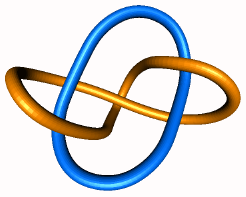
\includegraphics[width=0.75\linewidth]{./Pictures/Whiteheadlink}
			}
		\end{column}
  	\end{columns}
	%
	\pause
  	\begin{columns}
		\begin{column}[t]{.5\linewidth}	
			\begin{defblock}[Vorticity 2-form]
				$$
				\omega_{L} := \sum_{i=1}^n \omega_{L_i}, \qquad d\omega_L = 0
				$$
				($\omega_{ L_i}$ = \hyperlink{frame:poinduals}{Poincar\'e dual} associated to $L_i$)
			\end{defblock}
		\end{column}
		\begin{column}[t]{.5\linewidth}	
			\begin{defblock}[Velocity 1-form]
				\vspace{-.75em}
				$$
 					v_{ L} = \sum_{i=1}^n v_{L_i}, \qquad \qquad  dv_{L} = \omega_{ L}
				$$
				($v_{L_i} := \omega_{{\mathfrak a}_i}$ = \hyperlink{frame:poinduals}{Poincar\'e dual}  of a disc ${\mathfrak a}_i$ 
				bounded by 	$L_i$ \footnotesize{(Seifert surface)}) 
			\end{defblock}						
		\end{column}
  	\end{columns}
	%
	\pause
	%
	\tcbset{colback=white,
	colbacktitle=white,
	colframe=blue!70!black,
	boxrule=1pt,
	colupper=blue!70!black,
	arc=15pt,
	}
	\begin{tcolorbox}[sidebyside,righthand width=.7\linewidth]
		Thm: \cite{Miti2018}
		\tcblower
		$v_{L}$ is a {\it Hamiltonian 1-form}
		\\[.5em]
		\pause
		\hyperlink{frame:highorderlinking}{\footnotesize{(the same applies to every \emph{"higher velocity $1-form$})}}.
	\end{tcolorbox}	
	 

  
  \end{frame}
  \note[itemize]{
  	\item $G~=~SDiff_0(\mathbb{R}^3)$	(volume-preserving diffeomorphisms) encompasses ambient isotopies of knotted links (interpreted as singular vortices) and Euler evolution
	\item "instead as considering the knot we focus on its complementary"
	\item the context allows to understand certain knot theoretic quantities as hamiltonian forms
	\item $\omega_{ L_i}$ denote the Poincar\'e (or Thom) dual (class) associated to $L_i$: they are 2-forms localized in a 
 cross-section of a  suitable tubular neighbourhood $T_i$ around $L_i$ - with total fibre integral equal to one, or, as currents, 2-forms which are $\delta$-like on $L_i$
 
	\item $v_{L_i} := \omega_{{\mathfrak a}_i}$ is the Poincar\'e dual (class) of a disc ${\mathfrak a}_i$ bounding
$L_i$ (a Seifert surface for the trivial knot $L_i$). Precisely:
$$
\partial {\mathfrak a}_i = L_i, \qquad \qquad dv_{L_i} = d\omega_{{\mathfrak a}_i} = \omega_{L_i} = \omega_{\partial {\mathfrak a}_i},
$$
	\item
		Velocity 1-forms $v_i$ correspond (upon approximation of the associated Euler equation) to the so-called LIA (Linear Induction Approximation) or  {\it binormal evolution}
		of the ``vortex ring" $L_i$ (``orthogonal" to the discs ${\mathfrak a}_i$.
		
	\item Everything is up to choices of tubular neighbourhoods, Seifert surface and specific Poincar\'e dual.	
	
}
%------------------------------------------------------------------------------------------------





%----------------------------------------------------------------------------------------------------------------------------------
\end{document}
%----------------------------------------------------------------------------------------------------------------------------------
